\chapter{Stereo Reconstruction of Dense Surfaces to Walk on Rough Terrain} 
\label{Chap:3DReconstruction}

As we stated in figure \ref{Fig:GeneralDiagram} computer vision can be introduced (from hight to low level) in planning level, pattern generator level or whole-body motion level. In this chapter we will address the introduction of computer vision in the lowest level of robot motion generation: The Generalized Inverse Kinematics (GIK). This chapter differs from the previous ones in the sense that here we do not work at the pattern generator level. Consequently it is not directly related with the previous chapters of this thesis.

\section{Walking on Rough terrain}
% ~~~~~~~~~~~~~~~~~~~~~~~~~~~~~~~~~~~~~~~~~~~~~~~~~~~~~~~~~~~~~~~~~~~~~~~~~~~~~

In \citep{RamosIJHR2013} a proposal to walk on rough terrain was presented. It uses an inverse dynamics approach and a 3D reconstruction system to implement a compliant walking scheme. The inverse dynamics control scheme relies on a quadratic programming optimization solver and is used to let each foot go from its initial to its final position, controlling also the center of mass and the waist. A 3D model reconstruction of the ground is obtained through the robot cameras located on its head as a stereo vision pair. The model allows the system to know the ground structure where the swinging foot is going to step on. This is needed, e.g. for all the algorithms we mentioned in Chapters~\ref{Chap:Locomotion-Control}-\ref{Chap:Visual-Planning}. Thus, contact points can be handled to adapt the foot position to the ground conditions.

The inverse dynamics scheme is based in tree tasks: (i) a task for tracking the position of the CoM given by the Pattern Generator, (ii) a task to partially track the waist trajectory, this task controls the height of the waist as well as its orientation and, (iii) an interpolation task, this task takes the swinging foot from its initial position to its desired final position, the foot reacts in a compliant way if a contact is detected before arriving to the final position on the ground.

The contact points detection is done using a 3D model of the floor in front of the robot. This 3D model comes from a stereo reconstruction system which we will explain in more details in next section.

\section{Stereo reconstruction}

To perform the dense reconstruction of the floor surface in front of the robot, we rely on a real-time approach similar to KinectFusion algorithm proposed in~\citep{Newcombe2011}. This approach, originally developed for a RGB-D sensor, models 3-D surfaces as zero-valued level sets of functions defined over the workspace volume. These functions are referred to as truncated signed distance function (TSDF) and they are built incrementally, by integrating the depth measurements the sensor provides, frame after frame. TSDF are defined in the 3D space, and their value is the signed distance to the closest obstacle, as depicted in Fig.~\ref{Fig:TFDS}. Here, we extend this approach, initially proposed for RGB-D depth data, to disparity data generated from a stereo head. Although the stereo data is noisier than the one from RGB-D sensors, it is a passive sensor and can be used outdoors in sunlight conditions.


\begin{figure}
  \centering
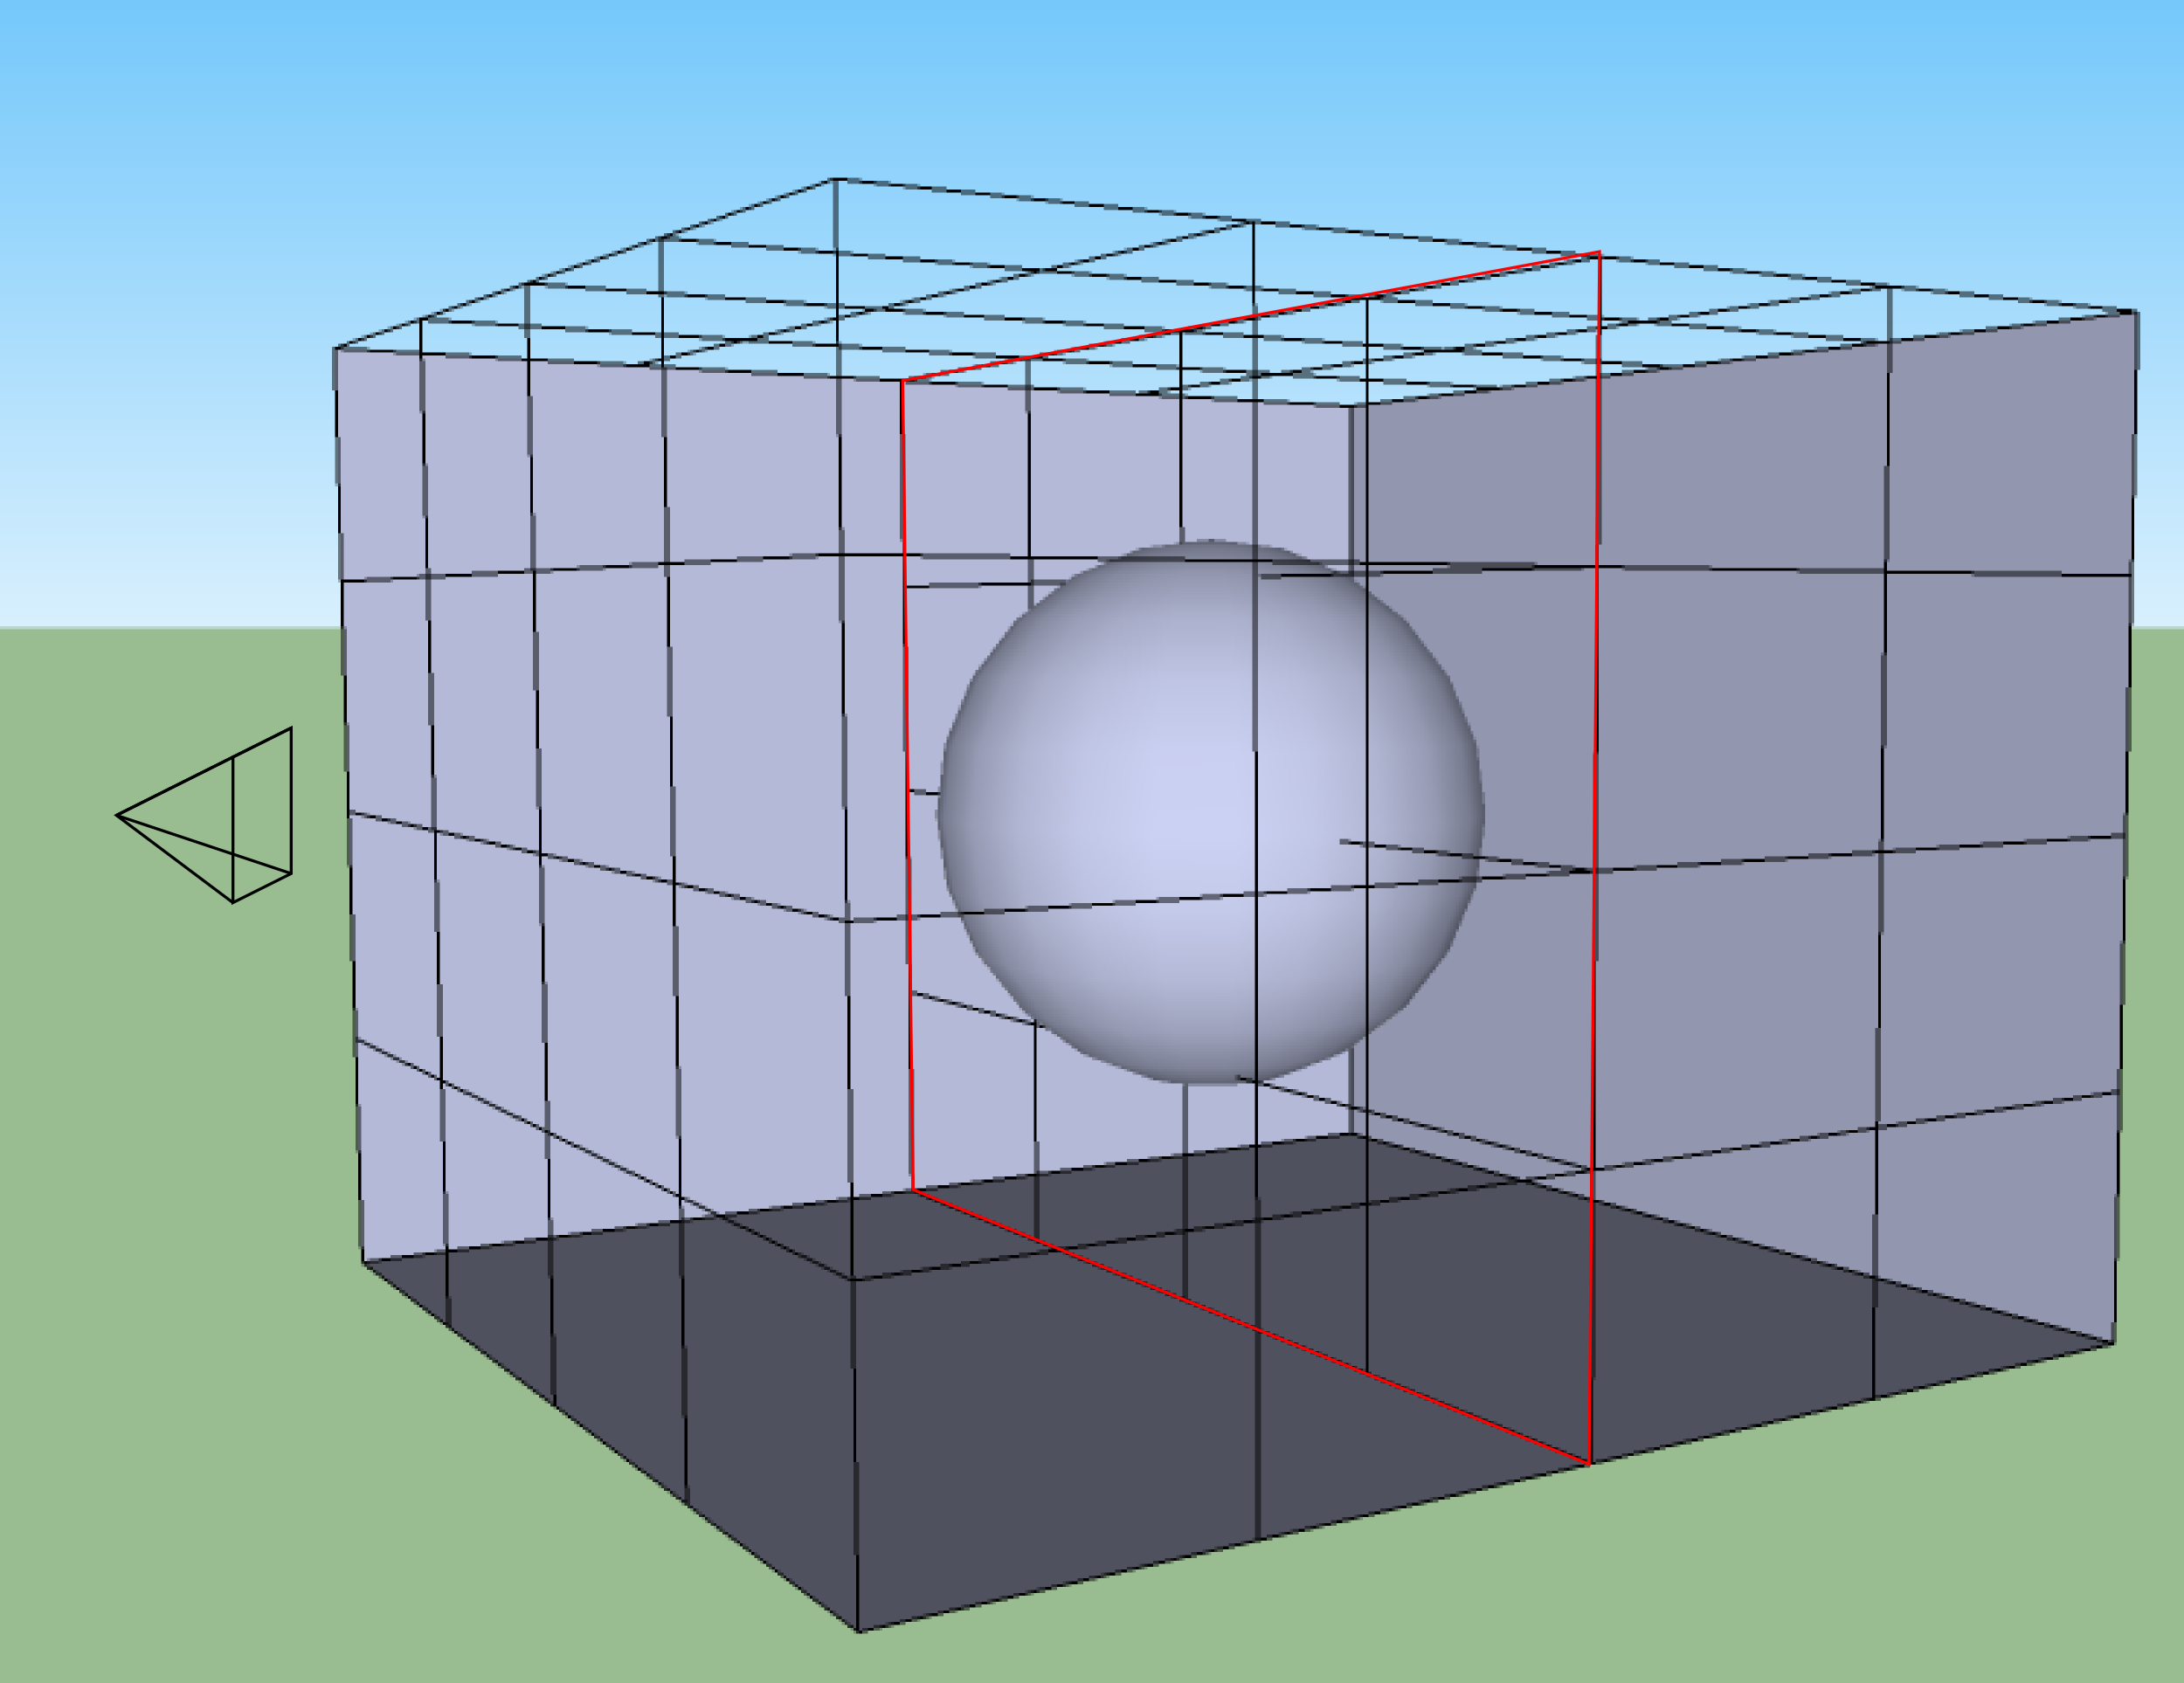
\includegraphics[scale=0.3]{Chap6-3D-Reconstruction/tfds}
      {\def\svgwidth{0.35\columnwidth}
        \subimport*{Chap6-3D-Reconstruction/}
                   {tfds2d.pdf_tex}}
      \caption[]{Consider the workspace of the left image. We discretize this space in a volumetric grid. And we assign to each voxel its truncated signed distance to the closest obstacle in the ray direction from the sensor, i.e. the surface, right image.}
      \label{Fig:TFDS}
\end{figure}


Consider, as in the previous sections, that $k$ is a discretized time index. The idea is to update a mathematical representation of the surface through a volumetric TSDF model (defined over a 3D grid), referred to as $F_k$. The basic steps for integrating one new set of disparity measurements at time $k$, to update $F_k$ and the corresponding surface, are the following ones: (i) Filter the raw depth measurements generated from the stereo head, $D_k$; here we used bilateral filtering for that purpose; (ii) From these filtered measurements and the prediction of the estimated surface at the previous step, estimate the transformation between the measured surface and the predicted one using the iterative closest point algorithm (ICP) and update the camera pose; (iii) Compute a volumetric grid formed from ``local'' TSDF values $F_{D_k}$, to which confidence weights $W_{D_k}$ are associated, and integrate them into the global volumetric grid $\{F_k,W_k\}$; (iv) Predict a new surface for the next iteration by using ray-casting over the zero-crossings of the fused global volumetric grid $\{F_k,W_k\}$. 

To use this algorithm with stereo data and generate local data $D_k$, a disparity map from a pair of rectified images is estimated, from which the depth map $D_k$ is derived, supposing the stereo rig is completely calibrated. The literature of algorithms that estimate disparity maps is huge, but since a real time one is needed for this application, the one proposed in~\citep{Geiger2010} has been used. This algorithm estimates a piece-wise disparity map using an initial sparse disparity map of high textured points as vertices that define a triangulation of the image. Then, the dense disparity map of each sub-region is estimated by using the initial, sparse disparity map as a prior in a probabilistic scheme. The steps of the reconstruction process are illustrated in Fig.~\ref{Fig:Reconstruction1}

\subsection{Pre-processing}
As mentioned above, it is necesary to apply a bilateral filter to the raw depth map to smooth it preserving the borders.
Then we project the pixel $\mathbf{u}$ to obtain a 3D the point $\mathbf{p}$. With the projection of all the pixels, we generate a vertex map,

\begin{equation}
 \mathbf{V}_k(\mathbf{u}) = D_k(\mathbf{u})\mathbf{K}^{-1}(\mathbf{u}),
\end{equation}

where $\mathbf{K}^{-1}(\mathbf{u})$ is the ray corresponding to the pixel $\mathbf u$. Since the depth measurements is a regular map, we can compute the normal vectors $\mathbf{N}_k(\mathbf{u})$ using the neighbours.



\subsection{Reconstruction}
The core of this algorithm is the computation and fusion of volumetric grids (i.e., the third step mentioned above). For a 3D point $\mathbf{p}$ expressed in the global frame $g$, its value in the current local volumetric grid $\{F_{D_k},W_{D_k}\}$ is computed as

$$
\left\{
\begin{array}{ccc}
F_{D_{k}}(\mathbf{p}) &=& \Psi (\lambda^{-1} \left \| \mathbf{t}_{g,k} - \mathbf{p}\right \| - D_k(\mathbf{x})), \\
W_{D_{k}}(\mathbf{p}) &\propto& \cos(\theta)/D_{k}(\mathbf{x}),
\end{array}
\right.
$$

with
$$
\Psi (\eta) =
\left \{
\begin{array}{cc}
\min(1,\frac{\eta}{\mu}) ~\text{sgn}(\eta) & \text{iff} ~ \eta \geq -\mu \\
\mbox{ null } & \mbox{ otherwise }
\end{array}
\right. , ~
\lambda = \left \| \mathbf{K}^{-1} [\mathbf{x}^\top 1]^\top \right \|,~
%\lambda = \left \| \mathbf{K}^{-1} \left[ \begin{matrix} \mathbf{x} \\ 1 \end{matrix} \right] \right \|,
$$

$\mu$ being a truncation distance (parameter of the algorithm), $\mathbf{x} = \pi([\mathbf{K},\mathbf 1] T^{-1}_{g,k} \mathbf{p}) \in \mathbb{R}^2$ being the image projection of $\mathbf p$. $\mathbf{K}$ is the $3\times 3$ matrix of intrinsic parameters of the camera, $\pi$ is the projection operator, $T_{g,k} = \left[ \begin{matrix} \mathbf{R}_{g,k} & \mathbf{t}_{g,k} \\ 0 & 1 \end{matrix} \right]$ the pose of the camera, at time $k$, in the global frame $g$, and $\theta$ the angle between the associated pixel ray direction and the surface normal.

The global volumetric grid at time $k$ is formed by the weighted average of all individual volumetric grids up to $k-1$. It can be shown that the optimal grid can be obtained incrementally using a simple point-wise on-line weighted average,

\begin{eqnarray*}
 F_k(\mathbf{p}) &=& \frac{W_{k-1}(\mathbf{p}) F_{k-1}(\mathbf{p}) + W_{D_{k}}(\mathbf{p}) F_{D_{k}}(\mathbf{p}) }{ W_{k-1}(\mathbf{p}) + W_{D_{k}}(\mathbf{p}) }, \\
 W_k(\mathbf{p}) &=& W_{k-1}(\mathbf{p}) + W_{D_{k}}(\mathbf{p}).
\end{eqnarray*}

With the previous equation we integrate incrementally the current measurement $\{ W_{D_{k}}(\mathbf{p}), F_{D_{k}}(\mathbf{p}) \}$ into the previous estimation of the grid $\{W_{k-1}(\mathbf{p}), F_{k-1}(\mathbf{p})\}$ to get current estimation of the grid $\{W_{k}(\mathbf{p}), F_{k}(\mathbf{p})\}$

\subsection{Surface prediction}
With the latest reconstruction we can compute a dense surface prediction by rendering the surface at the zero level of the TSDF on a virtual camera with the current estimation of $T_{g,k}$. This process will give us an estimated vertex and normal maps $\hat{\mathbf{V}}_k$ and $\hat{\mathbf{N}}_k$ that we will use in the camera pose estimation.
The vertex map is predicted by marching each ray $T_{g,k}K^{-1}\mathbf{u}$ stopping when a zero crossing ($+\nu e$ to $-\nu e$ for the visible side) is found from visible side to non-visible side indicating surface interface.
It may find a back face or exit of the working volume so there is no surface measurement in thar cases.
The normal map is computed as the gradient of the surface interface at $\mathbf{p}$ using numerical derivative:
\begin{equation}
 R_{g,k} \hat{\mathbf{N}}_g^k(\mathbf{u}) = \nu \nabla F(\mathbf{p}), \nabla F(\mathbf{p}) = \left [ \frac{\partial F}{\partial x}, \frac{\partial F}{\partial y}. \frac{\partial F}{\partial z} \right ]^T
\end{equation}
further this derivative is scaled.

For the marching ray, skipping, which provides useful acceleration is used. This is done by marching along the ray in steps of size $< \mu$ while values of $F(\mathbf{p})$ have $+ \nu e$ truncated values, so a step $\mu$ must pass at least one non-truncated value before stepping over the zero crossing.
Then to refine the intersection we take $F^+_t$ and $F^+_{t+\Delta t}$ which are the trilinearly interpolated values either side of the zero crossing along the ray $t$ and $t+\Delta t$ from its starting point.
Then the parameter at which the intersection occurs more precisely is computed,

\begin{equation}
t^* = t - \frac{\Delta t F^+_t}{F^+_{t+\Delta t} - F^+_t}
\end{equation}

so we have a vextex and normal maps in the interpolated point in the global frame.

\subsection{Sensor pose estimation}

The tracking is done by aligning the current surface measurement ($\mathbf{V}_k$,$\mathbf{N}_k$) against the model predicted from the previous frame ($\hat{\mathbf{V}}_{k-1}$,$\hat{\mathbf{N}}_{k-1}$).
In first place, projective data association algorithm is used to get a set of vetex correspondences $\{ \mathbf{V}_k(\mathbf{u}), \hat{\mathbf{B}}_{k-1}(\hat{\mathbf{u}}) \mid \Omega(\mathbf{u}) \neq null \}$ by computing the perspectively projected point $\hat{\mathbf{u}} = \pi(K \tilde{T}_{k-1.k} \dot{\mathbf{V}}_k(\mathbf{u}))$ using an estimate of the frame transform and testing the predicted and measured vertex and normal for compatibility.

An iterative solution $\tilde{T}^z_{g,k}$ is obtained by minimizing a linearized version of the global point-plane energy around the previous estimate $\tilde{T}^{z-1}_{g,k}$. Using the small angle assumption for an incremental transform $\tilde{T}^z_{inc}$, the update is $\tilde{T}^z_{g,k} = \tilde{T}^z_{inc}\tilde{T}^{z-1}_{g,k}$.
The minimization is done using the incremental point transfer $\tilde{\mathbf{V}}^g_k(\mathbf{u}) = \tilde{T}^{z-1}_{g,k} \dot{\mathbf{V}}_k(\mathbf{u})$. 
Arranging the parameters of the transformation as $ \mathbf{x} = (\beta,\gamma,\alpha,t_x,t_y.t_z)^T$ we can write
\begin{equation}
\tilde{T}^z_{g,k} \dot{\mathbf{V}}_k(\mathbf{u}) = \tilde{R}^z \tilde{\mathbf{V}}^g_k(\mathbf{u}) + \tilde{\mathbf{t}}^z = \mathbf{G}(\mathbf{u})\mathbf{x} + \tilde{\mathbf{V}}^g_k(\mathbf{u}).
\end{equation}

An iteration is obtained by solving

\begin{equation}
\underset{\mathbf{x} \in  \mathbb{R}^6 }{min} \sum_{\Omega_k (\mathbf{u}) \neq null} \left \| E \right \|^2_2
\end{equation}

\begin{equation}
 E = \tilde{\mathbf{N}}^g_{k-1}(\mathbf{u})^T \left( \mathbf{G}(\mathbf{u})\mathbf{x} + \tilde{\mathbf{V}}^g_k(\mathbf{u}) - \hat{\mathbf{V}}^g_{k-1}(\hat{\mathbf{u}}) \right)
\end{equation}

The minimum can be found analytically by derivating the objective function and setting to zero. A $6 \times 6$ symmetric linear system is generated for each correspondence. Solving for $\mathbf{x}$, we obtain $\tilde{T}^z_{g,k}$.
The data association and pose estimation is embedded into a coarse to fine framework using the bottom 3 levels of the vertex and normal maps pyramid, the camera pose results of the last iteration.

\section{Results}

For the implementation, we adapted the Kinfu algorithm which is provided with the Point Cloud Library (PCL). We also used the stereo matching algorithm which is provided in the authors web page \footnote{http://www.cvlibs.net/software/libelas/}. We made the experiments with the stereo rig which is in the head of the HRP-2 humanoid robot. In order to do that, we used the Robot Operating System (ROS) framework as a middleware to link the different parts.

In Fig. \ref{Fig:Reconstruction1} we depict the input and output of the stages of the algorithm. In Figs. \ref{Fig:Reconstruction1}, \ref{Fig:Reconstruction2} we show the results with the scene of flat floor and some objects on it, like books and small boxes. In Fig. \ref{Fig:Reconstruction3} we tested the algorithm in a stairs scene with the small objects as well. Finally, in Fig. \ref{fig.robot-walking-obstacle} we depict a fully dynamic simulation of the HRP-2 robot while walking on rough terrain using the reconstruction system presented in this chapter.

\begin{figure}[h] \centering
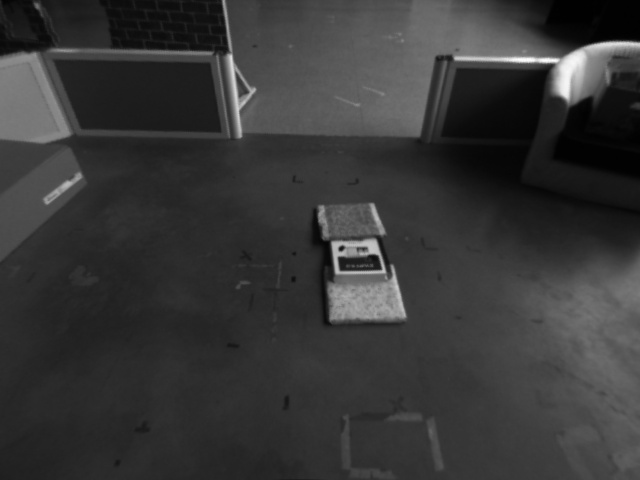
\includegraphics[scale=0.25]{Chap6-3D-Reconstruction/left0001}
\hspace{0.2cm}
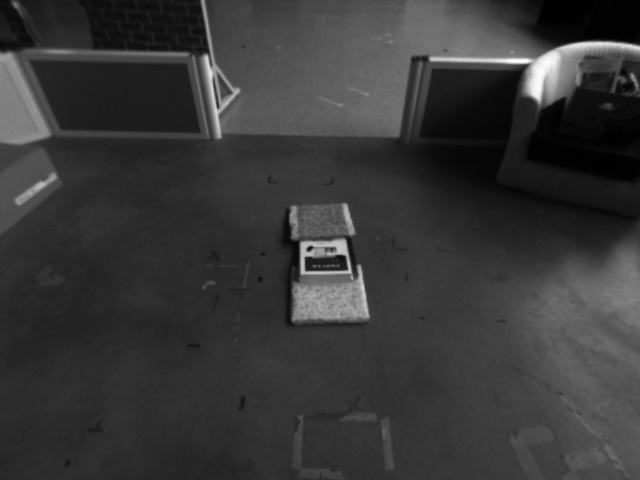
\includegraphics[scale=0.25]{Chap6-3D-Reconstruction/right0001}
\vspace{0.2cm}
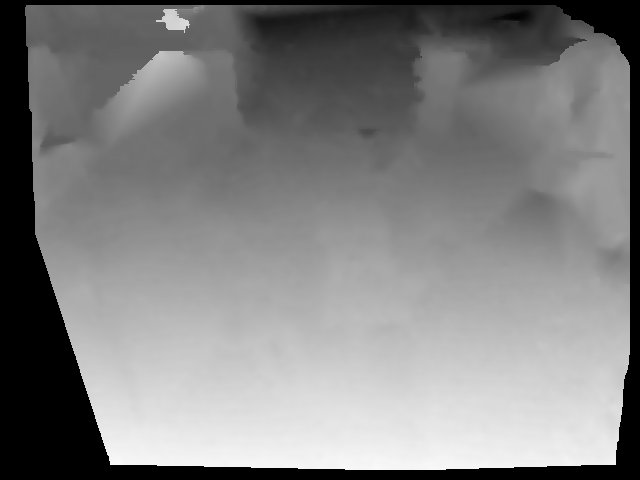
\includegraphics[scale=0.37]{Chap6-3D-Reconstruction/left0001_disp}
\vspace{0.2cm}
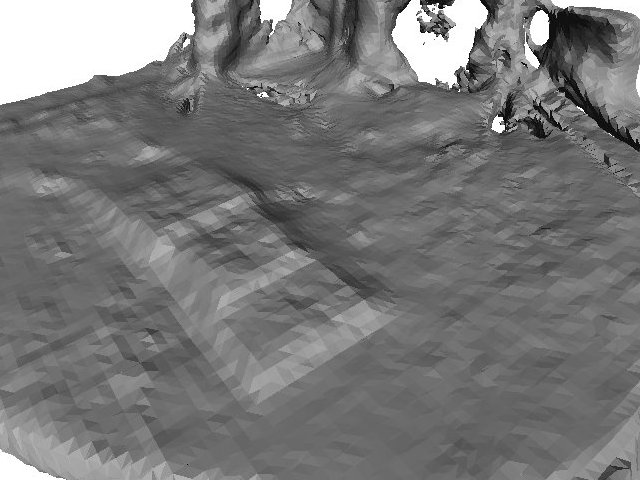
\includegraphics[scale=0.5]{Chap6-3D-Reconstruction/snapshot02}
\caption[]{From a pair of images of the scene in front of the robot
(left) we estimate a dense disparity map (middle) and from this
disparity map we estimate a dense surface integrating the previous
frames into the volumetric grid.}
\label{Fig:Reconstruction1}
\end{figure}


\begin{figure}[h]
\centering
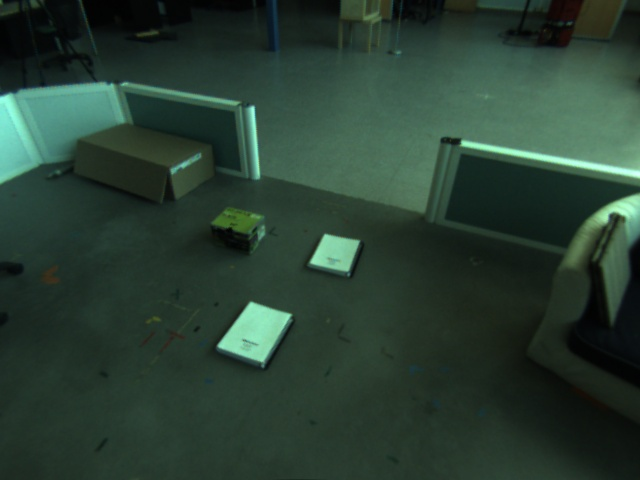
\includegraphics[scale=0.5]{Chap6-3D-Reconstruction/frame0005}
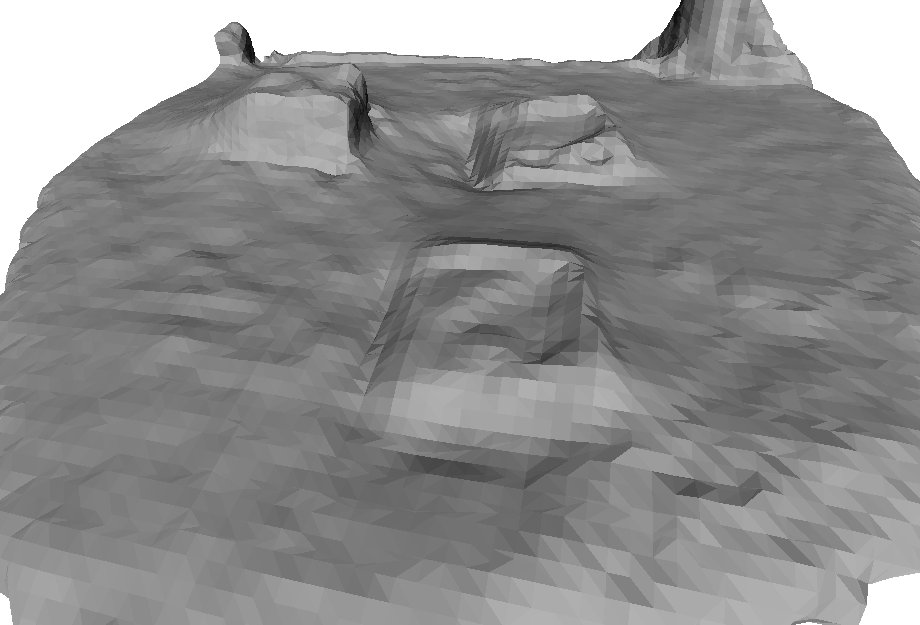
\includegraphics[scale=0.5]{Chap6-3D-Reconstruction/snapshot01}
\caption[]{Reconstruction of a scene of flat floor with small objects on it like books and boxes.}
\label{Fig:Reconstruction2}
\end{figure}

\begin{figure}[h]
\centering
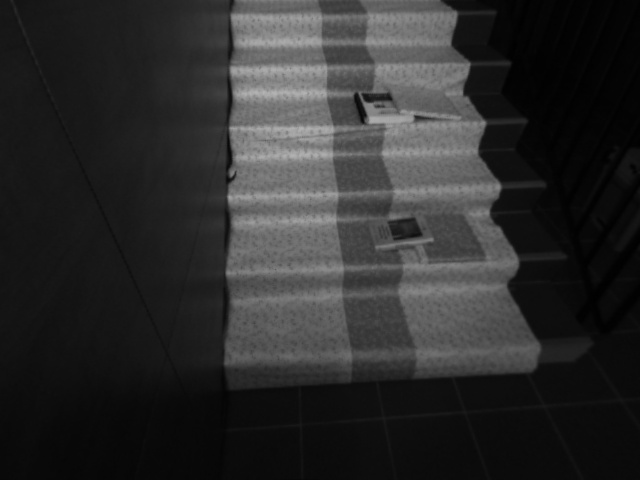
\includegraphics[scale=0.5]{Chap6-3D-Reconstruction/left0003}
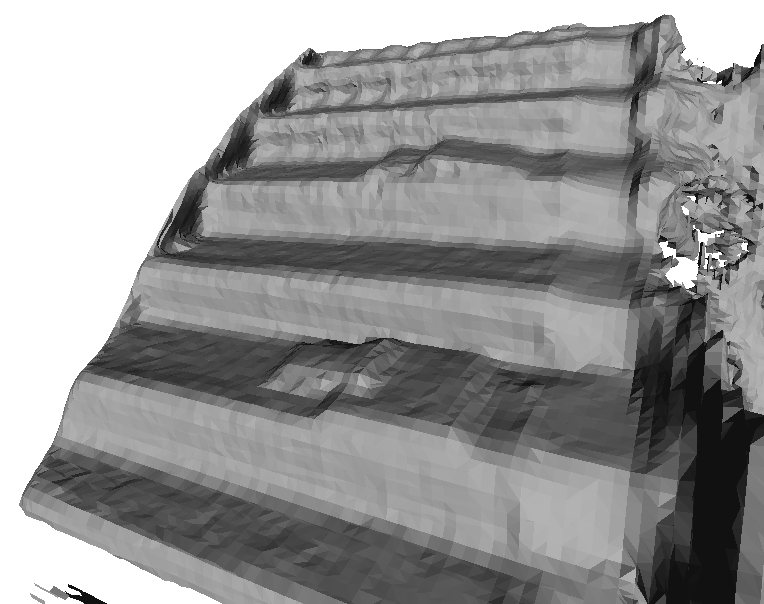
\includegraphics[scale=0.57]{Chap6-3D-Reconstruction/snapshot00}
\caption[]{Reconstruction of a stairs scene with some objects on it.}
\label{Fig:Reconstruction3}
\end{figure}

\begin{figure*}
\centering \footnotesize
\subfigure[\footnotesize \label{fig.w1}]{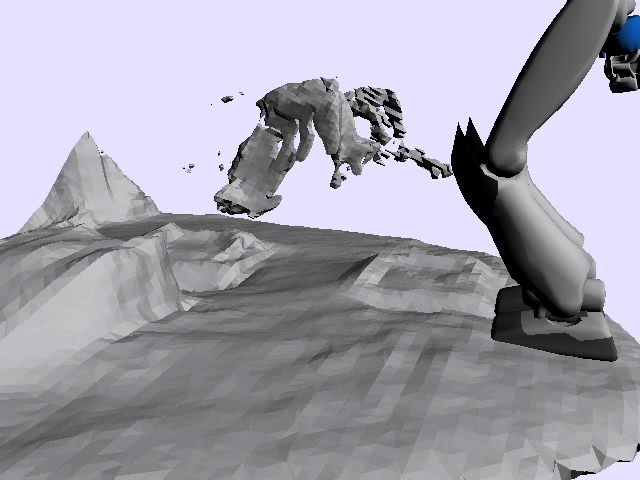
\includegraphics[width=0.35\linewidth ]{Chap6-3D-Reconstruction/robot-obstacle1.png}} ~  %\hfill
\subfigure[\footnotesize \label{fig.w2}]{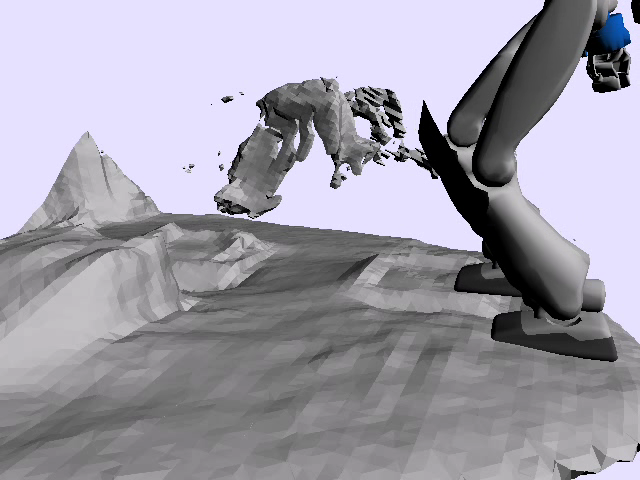
\includegraphics[width=0.35\linewidth]{Chap6-3D-Reconstruction/robot-obstacle2}} \\   %\hfill
\subfigure[\footnotesize \label{fig.w3}]{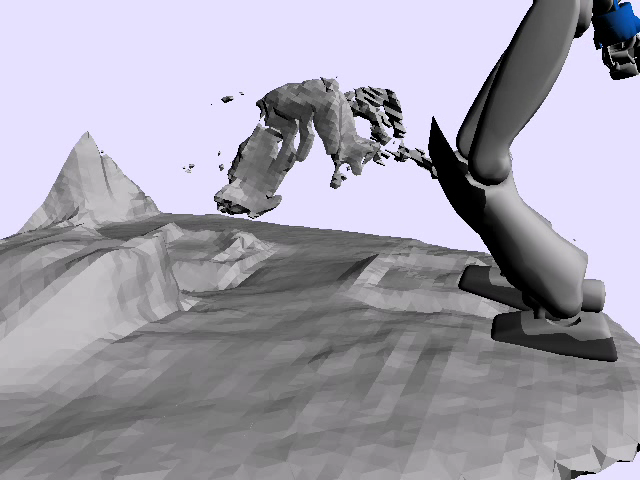
\includegraphics[width=0.35\linewidth]{Chap6-3D-Reconstruction/robot-obstacle3}}  ~ %\hfill
\subfigure[\footnotesize \label{fig.w3}]{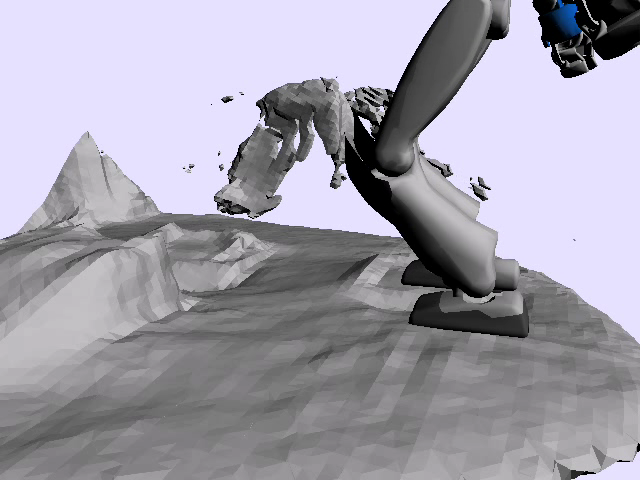
\includegraphics[width=0.35\linewidth]{Chap6-3D-Reconstruction/robot-obstacle4}} \\  %\hfill
\subfigure[\footnotesize \label{fig.w3}]{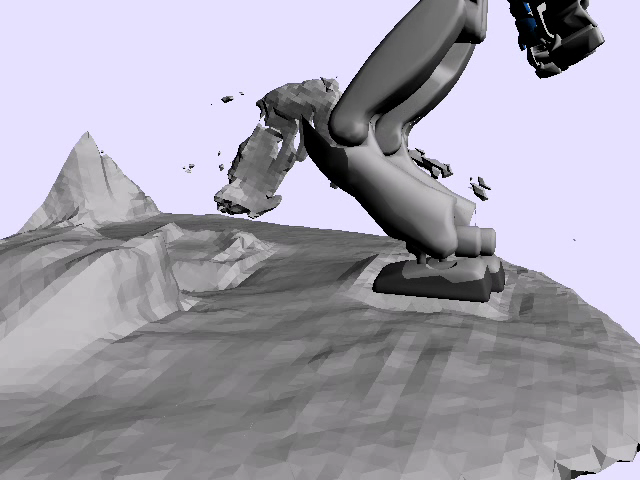
\includegraphics[width=0.35\linewidth]{Chap6-3D-Reconstruction/robot-obstacle5}} ~   %\hfill
\subfigure[\footnotesize \label{fig.w3}]{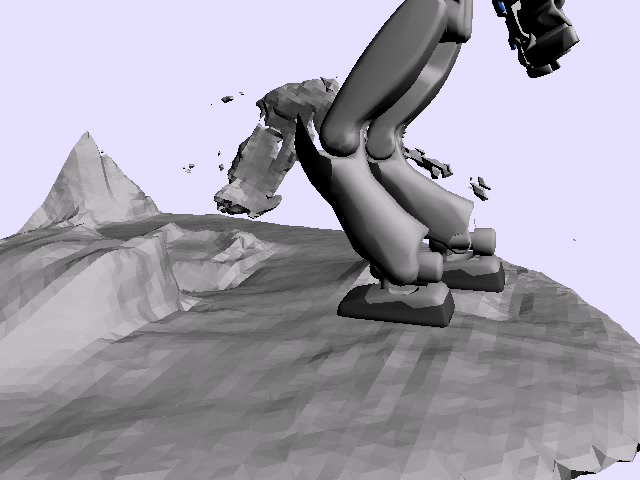
\includegraphics[width=0.35\linewidth]{Chap6-3D-Reconstruction/robot-obstacle6}}
\caption{HRP-2 walking on an obstacle.}
\label{fig.robot-walking-obstacle}
\end{figure*}

\section{Conclusion}

In this chapter we presented the connection of existing algorithms of efficient stereo matching and 3D reconstruction to be used in a more complex system to make the robot walk on rough terrain. This connection was done over ROS and tested successfully with scenes of flat floor and stairs with small objects on them. The output of this algorithm provides a model of the world to a control system which implements a compliant walking scheme.